\section[VHSIC Hardware Description Language (VHDL)]{
  VHSIC Hardware Description Language (VHDL)
  % \texttt{VHDL}: Very high-speed integrated circuits program
  % Hardware Description Language
}

\subsection{Basic syntax and identifiers}
In VHDL an identifier is a case insensitive string composed of
\texttt{A-Z a-z 0-9 \_} that
\begin{itemize}
  \item is not a keyword,
  \item does not start with a number or \texttt{\_},
  \item does not have two or more \texttt{\_} in a row.
\end{itemize}
Expressions are terminated by a semicolon \texttt{;}.
Two dashes in a row cause the rest of the line to be interpreted as a comment.
\begin{lstlisting}[language=vhdl]
expression; -- comment
\end{lstlisting}

\subsection{Structure and Libraries}
The VHDL code is organized into \emph{libraries} declared with the
\vhdl{library} keyword. The library of your code is called \texttt{work},
standard features (\texttt{bit}, \texttt{integer}, \ldots) are found in
\texttt{std}, and IEEE standard parts are in \texttt{ieee}. \texttt{work} and
\texttt{std} are always implicit and must not be declared.
\begin{lstlisting}[language=vhdl]
library `\reqph{library name}`;
\end{lstlisting}
Once declared a library is composed of \emph{packages}, which can contain
elements (constants, entities, \ldots). To access the elements the syntax is 
\begin{lstlisting}[language=vhdl]
`\reqph{library}`.`\reqph{package}`.`\reqph{element}`;
\end{lstlisting}
To avoid having to write a long name every time it is possible to import names
using
\begin{lstlisting}[language=vhdl]
use `\reqph{library}`.`\reqph{element or {\tt all}}`;
use `\reqph{library}`.`\reqph{package}`.`\reqph{element or {\tt all}}`;
\end{lstlisting}

\subsection{Entities and Architectures} \label{sec:vhdl:entities-arch}
In VHDL the concept of \emph{entity} describes a black box of which only
inputs and outputs are known. The internals of an entity are described through
an \emph{architecture}. There can be multiple architectures for a single entity.

\begin{figure}[h]
  \centering
  \begin{tikzpicture}[
      font = \ttfamily,
      node distance = 1mm,
      pin/.style = {
        draw = black, fill = white, circle, thick,
        inner sep = 0pt, minimum size = 2mm,
      },
    ]
    \node[
      rectangle, draw = black, thick, fill = gray!20!white,
      minimum width = 4.5cm, minimum height = 4cm,
    ] (entity) {};

    \node[anchor = south west] at (entity.north west) {Entity};

    \foreach \x in {1,2,3}{
      \node[
        rectangle, draw = black, thick, fill = white,
        minimum width = 3.5cm, minimum height = .75cm,
      ] (arch\x) at ($(entity.north) + (0, -1 * \x)$) {Architecture \x};
    }

    \foreach \x in {1,...,4}{
      \draw[thick]
        ($(entity.north west) - (0, .75 * \x)$) 
        node[pin] {} to ++(-.75, 0) node (pinl\x) {};

      \draw[thick]
        ($(entity.north east) - (0, .75 * \x)$)
        node[pin] {} to ++(.5, 0) node (pinr\x) {} ;
    }

    \node[right] at (pinr1) {Pin};
  \end{tikzpicture}
  \caption{An entity is a black box, that can have multiple architectures.}
\end{figure}

Entities are declared with \vhdl{port()} that may contain a list of pins. Pins
have a mode that can be \vhdl{in} input (only LHS\footnote{Left hand side}),
\vhdl{out} output (only RHS\footnote{Right hand side}), \vhdl{inout}
bidirectional or \vhdl{buffer} that can stay both on LHS and RHS. The usage of
the latter is discourareged in favour of an internal signal.
\begin{lstlisting}[language=vhdl]
entity `\reqph{name}` is
  port(
    `\reqph{pin}` : `\reqph{mode} \reqph{type}`;
    `\optionalph{more pins}`;
    `\reqph{pin}` : `\reqph{mode} \reqph{type}`
  );
end entity `\optionalph{name}`;
\end{lstlisting}

Architectures are normally named after the design model, examples are
\texttt{behavioral}, \texttt{structural}.
\begin{lstlisting}[language=vhdl]
architecture `\reqph{name}` of `\reqph{entity}` is
  -- declare used variables, signals and component types
begin
  -- concurrent area
end architecture `\optionalph{name}`;
\end{lstlisting}

\subsection{Type system}
\subsubsection{Electric types}
VHDL provides some types such as
\begin{itemize}
  \item \vhdl{boolean} true or false,
  \item \vhdl{bit} 0 or 1,
  \item \vhdl{bit_vector} one dimensional array of bits,
  \item \vhdl{integer} 32-bit binary representation of a value.
\end{itemize}
From external (standard) libraries other types are available:
\begin{itemize}
  \item \vhdl{std_logic} advanced logic with 9 states,
  \item \vhdl{std_ulogic} same as the previous but \emph{unresolved}.
\end{itemize}
The above are from the \vhdl{ieee.std_logic_1164} library, and can take the
values described in table \ref{tab:std-logic-1164-types}.
\begin{table}[h]
  \centering
  \begin{tabularx}{\linewidth}{>{\ttfamily}c l X}
    \toprule
    \textrm{Value} & Meaning & Usage \\
    \midrule
    U & Uninitialized  & In the simulator \\
    X & Undefined      & Simulator sees a bus conflict \\
    0 & Force to 0     & Low state of outputs \\
    1 & Force to 1     & High state of outputs \\
    Z & High Impedance & Three state ports \\
    W & Weak Unknown   & Simulator sees weak a bus conflict \\
    L & Weak Low       & Open source outputs with pull-down resistor \\
    H & Weak High      & Open drain output with pull-up resistor \\
    - & Don't care     & Allow minimization \\
    \bottomrule
  \end{tabularx}
  \caption{
    Possible values for \vhdl{std_logic} signals.
    \label{tab:std-logic-1164-types}
  }
\end{table}
For the \emph{resolved} types, i.e. \vhdl{std_logic} types, when a signal is
multiply driven the conflict is resolved according to table
\ref{tab:std-logic-1164-resolve}.  Unresolved types will give a synthesization
error.  A good example is a tri-state bus: 
\begin{lstlisting}[language=vhdl]
architecture tristate of buscontrol is
begin
  bus_read: inp <= bus_io;

  bus_write: process(enable, oup)
  begin
    bus_io <= (others => 'Z');
    if enable = '1' then
      bus_io <= oup;
    end if;
  end process;
end architecture tristateout;
\end{lstlisting}
\begin{table}[h]
  \centering
  {
    \ttfamily
    \begin{tabular}{c|ccccccccc} 
      \toprule
      & U & X & 0 & 1 & Z & W & L & H & - \\
      \midrule
      U & U & U & U & U & U & U & U & U & U \\
      X & U & X & X & X & X & X & X & X & X \\
      0 & U & X & 0 & X & 0 & 0 & 0 & 0 & X \\
      1 & U & X & X & 1 & 1 & 1 & 1 & 1 & X \\
      Z & U & X & 0 & 1 & Z & W & L & H & X \\
      W & U & X & 0 & 1 & W & W & W & W & X \\
      L & U & X & 0 & 1 & L & W & L & W & X \\
      H & U & X & 0 & 1 & H & W & W & H & X \\
      - & U & X & X & X & X & X & X & X & X \\
      \bottomrule
    \end{tabular}
  }
  \caption{
    Resolution table when a \vhdl{std_logic} signal is multiply driven.
    \label{tab:std-logic-1164-resolve}
  }
\end{table}

\subsubsection{Arithmetic types}
For arithmetic operations two more types \texttt{signed} and \texttt{unsigned}
(as well as their unresolved equivalents \texttt{u\_signed} and
\texttt{u\_unsigned}) can be imported (together with many others for ex.
\texttt{natural}) from the library \texttt{ieee.numeric\_std}. Arithmetic types
support the operations in table \ref{tab:arithmetic-type-ops}.
\begin{table}[h]
  \begin{tabularx}{\linewidth}{>{\ttfamily}c p{.3\linewidth} X}
    \toprule
    \textrm{Syntax} & Operator & Note \\
    \midrule
    + & Addition \\
    - & Subtraction \\
    abs() & Absolute value \\
    * & Multiplication \\
    / & Division & Typically not available\\
    ** & Power & Only powers of 2 \\
    mod & Modulo & Only modulo of \(2^k\) \\
    rem & Remainder & Only of division by \(2^k\) \\
    = & Equality \\
    /= & Inequality \\
    <\textrm{,} > & Lower, greater \\
    <=\textrm{,} >= & Lower, greater or equal & Same the assignment operator, however it is always clear from context. \\
    \bottomrule
  \end{tabularx}
  \caption{
    Arithmetic operations from the \texttt{numeric\_std} library.
    \label{tab:arithmetic-type-ops}
  }
\end{table}

\subsubsection{Array type}
Arrays types (fields) of other types can be define with the following.
\begin{lstlisting}[language=vhdl]
type `\reqph{name}` is array (`\reqph{upper limit}` downto `\reqph{lower limit}`) of `\reqph{base type}`;
\end{lstlisting}

\subsubsection{Custom enumeration types}
It is possible to create custom types, usually to create state machines.
\begin{lstlisting}[language=vhdl]
type `\reqph{name}` is (`\reqph{identifier}`, `\reqph{identifier}`, `\ph{\ldots}`);
\end{lstlisting}

\subsubsection{Physical types}
For variables that represent physical dimensions it is possible to create
values with units with the following:
\begin{lstlisting}[language=vhdl]
type `\reqph{name}` is range `\reqph{min}` to `\reqph{max}`
units
  `\reqph{base unit}`;
  `\optionalph{multiples of base unit}`;
end units;
\end{lstlisting}
for example:
\begin{lstlisting}[language=vhdl]
type CAPACITANCE is range 0 to 1E30
units
  pf;
  nf = 1000 pf;
  uf = 1000 nf;
  mf = 1000 uf;
end units;
\end{lstlisting}

\subsubsection{Reisizing vectors}
VHDL has a function
\begin{lstlisting}[language=vhdl]
function resize(arg: signed; new_size: natural) return signed;
\end{lstlisting}
that allow to reisze vector types. When resizing a vector of signed type to a
higher number of bits the \vhdl{resize} function cleverly fills the extra bits
1s or 0s to not mess up the two's complement. Toghether with the \vhdl{resize}
function an often used feature is the \vhdl{'length} attriubte, that returns
the size (in bits) of the identifier.
\begin{lstlisting}[language=vhdl]
y <= resize(a, y'length);
\end{lstlisting}

\subsubsection{Type casting and conversion}
When two signals have the same underlying type it is always possible to perform
a \emph{type cast} using the following syntax.
\begin{lstlisting}[language=vhdl]
`\reqph{destination}` = `\reqph{type name}`(`\reqph{source}`);
\end{lstlisting}
For example:
\begin{lstlisting}[language=vhdl]
architecture behavoral of cast_example
  signal a_int, b_int : 
    std_logic_vector(3 downto 0);
  signal s_int : unsigned(3 downto 0);
begin
  s_int <= unsigned(a_int) 
         + unsigned(b_int);
end architecture;
\end{lstlisting}
When the conversion is between signals with a different underlying type it is a
(potentially lossy) \emph{type conversion}. The syntax for a conversion is:
\begin{lstlisting}[language=vhdl]
`\reqph{destination}` = to_`\reqph{type name}`(`\reqph{source}`);
\end{lstlisting}
\begin{figure}[h]
  \pgfdeclarelayer{background}
  \pgfsetlayers{background,main}
  \begin{tikzpicture}[
      font = \small\ttfamily,
      box/.style = {
        draw, thick, black, fill = lightgray!20,
        rounded corners = 5pt,
        align = center,
        outer sep = 1mm,
        inner sep = 3mm,
      },
      func/.style = {
        black,
        font = \small\ttfamily,
        fill = white,
        pos = .5,
      },
      afunc/.style = {
        func, fill = hsr-blue20,
      },
    ]
    \matrix[nodes = box, row sep = 2cm, column sep = 3mm]{
      & \node (slv) {\vhdl{std_logic_vector}}; \\
      \node (s) {\vhdl{signed}}; & & \node (u) {\vhdl{unsigned}}; \\[3mm]
      & \node (int) {\vhdl{integer}}; \\
    };

    \begin{pgfonlayer}{background}
      \coordinate (sr) at ($(s.south west)-(.2,.2)$);
      \coordinate (ur) at ($(u.south east)+(.2,-.2)$);
      \coordinate (slvr) at ($(slv.north)+(0,.2)$);

      \fill[hsr-blue20]
        (sr) to (ur) to (ur) |- (slvr) to (slvr) -| (sr) to cycle;

      \node[above, hsr-blue80] at (slvr) {array types};
    \end{pgfonlayer}

    \draw[thick, ->]
      (slv) edge[out = 180, in = 90] node[afunc] {\vhdl{signed()}} (s)
      (slv) edge[out = 0, in = 90] node[afunc] {\vhdl{unsigned()}} (u)
      %
      (u) edge[out = 150, in = -60] (slv)
      (s) edge[out = 30, in = -120] node[
        afunc, pos = .7, xshift = 5mm,
      ] {\vhdl{std_logic_vector()}} (slv)
      %
      (u) edge[out = 210, in = 60] (int)
      (s) edge[out = -30, in = 120] node[
        func, pos = .62, xshift = 5mm,
      ] {\vhdl{to_integer()}} (int)
      %
      (int) edge[out = 180, in = 270] node[
        func, pos = .85, xshift = 4mm,
      ] {\vhdl{to_signed(}\reqph{v},\reqph{len})} (s)
      (int) edge[out = 0, in = 270] node[
        func, pos = .55, xshift = -3mm,
      ] {\vhdl{to_unsigned(}\reqph{v},\reqph{len})} (u)
      %
      (s) edge[out = 10, in = 170] node[afunc, above] {\vhdl{unsigned()}} (u)
      (u) edge[out = 195, in = -15] node[afunc, above = 1mm] {\vhdl{signed()}} (s)
    ;
  \end{tikzpicture}
\end{figure}

\subsection{Declarations} \label{sec:vhdl:declarations}
Before a \vhdl{begin} -- \vhdl{end} block, there is usually a list of declarations.
A self evident examples are \emph{constants}.
\begin{lstlisting}[language=vhdl]
constant `\reqph{name}` : `\reqph{type}` := `\reqph{value}`;
\end{lstlisting}

Next, \emph{signals} and \emph{variables}. Signals are wires, they can only be
connected and do not have an initial state. Variables can be assigned like in
software, but can cause the synthesization of an unwanted D-Latch.

\begin{lstlisting}[language=vhdl]
signal `\reqph{name}`, `\optionalph{name, \ldots}` : `\reqph{type}`;

variable `\reqph{name}`, `\optionalph{name}`, `\optionalph{\ldots}` : `\reqph{type}`;
variable `\reqph{name}` : `\reqph{type}` := `\reqph{expression}`;
\end{lstlisting}

For the hierarchical designs, when external entities are used, they must be
declared as components. The \vhdl{port()} expression must match the entity
declaration.
\begin{lstlisting}[language=vhdl]
component `\reqph{entity name}` is
  port(
    `\optionalph{list of pins}`
  );
end component;
\end{lstlisting}
For entities with multiple architectures, it is possible to choose which
architecture is used with the following expression.
\begin{lstlisting}[language=vhdl]
for `\reqph{label or {\tt all}}`: use entity `\reqph{library}`.`\reqph{entity}`(`\reqph{architecture}`);
\end{lstlisting}

\subsection{Concurrent Area} \label{sec:vhdl:concurrent}
\begin{figure}[h]
  \centering
  \begin{tikzpicture}[
      font = \ttfamily,
      node distance = 1mm,
      pin/.style = {
        draw = black, fill = white, circle, thick,
        inner sep = 0pt, minimum size = 2mm,
      },
      component/.style = {
        draw = black, thick, fill = white, rectangle,
        minimum width = 18mm, minimum height = 12mm,
        align = center,
      },
    ]

    \node[
      draw = black, rectangle, fill = gray!20!white, thick,
      minimum width = .75\linewidth, minimum height = 4cm,
    ] (arch) {};

    \node[anchor = south west] at (arch.north west) {Architecture};

    \node[pin] (clk) at ($(arch.north west) - (0,1)$) {};
    \node[pin] (a) at ($(clk) - (0,1)$) {};
    \node[pin] (b) at ($(a) - (0,1)$) {};
    \node[pin] (y) at ($(arch.north east) - (0,1)$) {};

    \node[left = of clk] {clk};
    \node[left = of a] {a};
    \node[left = of b] {b};
    \node[right = of y] {y};

    \node[component] (c1) at ($(clk) + (2,-.2)$) {Process};
    \node[component] (c2) at ($(c1) + (.2,-1.8)$) {Component\\ (entity)};
    \node[
      component, minimum width = 0mm, minimum height = 0mm,
    ] (c3) at ($(c1) + (2.6,-.2)$) {Logic\\ Gate};

    \draw[thick]
      (clk)     to[out = 0, in = 180] ($(c1.west) + (0,.2)$)
      (a)       to[out = 0, in = 180] ($(c1.west) - (0,.2)$)
      (b)       to[out = 0, in = 180] (c2.west)

      (c1.east) to[out = 0, in = 180] ($(c3.west) + (0,.2)$)
      (c2.east) to[out = 0, in = 180] ($(c3.west) - (0,.2)$)
      (c3.east) to[out = 0, in = 180] (y)
      ;

  \end{tikzpicture}
  \caption{
    In the concurrent area statements are not interpreted sequentially.
  }
\end{figure}

In the architecture between \vhdl{begin} and \vhdl{end}, the expressions
are \emph{not} read sequentially, everything happens at the same time.
Statements inside the concurrent area optionally have a label.
\begin{lstlisting}[language=vhdl]
`\optionalph{label}`: `\reqph{concurrent statement}`;
\end{lstlisting}
In the concurrent area signals, components and processes can be used to create
a logic.

\subsubsection{Signal assignment and simple gates}
Signals are assigned using \vhdl{<=}.
\begin{lstlisting}[language=vhdl]
`\optionalph{label}`: `\reqph{signal}` <= `\reqph{expression}`;
\end{lstlisting}
Simple logic functions such as \vhdl{not}, \vhdl{and}, \vhdl{or}, \vhdl{xor},
etc. can be used.
\begin{lstlisting}[language=vhdl]
 y <= (a and s) or (b and not(s));
\end{lstlisting}

\subsubsection{Aggregates}
For vector types it is possible to create a value out of multiple signals.
\begin{lstlisting}[language=vhdl]
`\reqph{vector}` <= (
  `\reqph{index}`  => `\reqph{source or value}`,
  `\reqph{index}`  => `\reqph{source or value}`,
  `\optionalph{\tt others}` => `\reqph{source or value}`
);
\end{lstlisting}
\begin{lstlisting}[language=vhdl]
-- declaration
signal data : bit_vector(6 downto 0);
signal a, b : bit;
\end{lstlisting}
\begin{lstlisting}[language=vhdl]
-- concurrent
data = (1 => a, 0 => b, others => '0')
\end{lstlisting}

\subsubsection{Selective and conditional assignment}
Higher level conditions can be written in two ways. 
\begin{lstlisting}[language=vhdl]
-- using when
`\optionalph{label}:` y <= `\reqph{source}` when `\reqph{condition}` else
     `\reqph{source}` when `\reqph{condition}` else
     `\reqph{source}` when `\reqph{condition}`;
\end{lstlisting}
\begin{lstlisting}[language=vhdl]
-- using with
`\optionalph{label}`: with `\reqph{signal}` select `\reqph{dest}` <= 
  `\reqph{source}` when `\reqph{value}`,
  `\reqph{source}` when `\reqph{value}`,
  `\reqph{source}` when others;
\end{lstlisting}

\subsubsection{Components} \label{sec:vhdl:components}
External components that have been previously declared can be used with the
\vhdl{port map(}\reqph{assignments}\texttt{)} syntax. For example:
\begin{lstlisting}[language=vhdl]
-- declaration
component flipflop is
  port(
    clk, set, rst : in  std_ulogic;
    Q, Qn         : out std_ulogic 
  );
end component flipflop;

signal clk_int, a, b : in  std_ulogic;
signal y, z          : out std_ulogic;
\end{lstlisting}
\begin{lstlisting}[language=vhdl]
-- concurrent
u1: component flipflop
  port map(
    clk => clk_int,
    set => a,
    rst => b,
    Q   => y,
    Qn  => z
  );

\end{lstlisting}

\subsubsection{Processes}
For more sophisticated logic VHDL offers a way of writing sequential statements
called \emph{process}.
\begin{lstlisting}[language=vhdl]
`\optionalph{label}:` process (`\optionalph{sensitivity list}`)
-- declarations
begin
  -- sequential statements
end process;
\end{lstlisting}
Processes have a \emph{sensitivity list} that can be empty.  When a signal in
the sensitivity list changes state, the process is executed.  With an empty
sensitivity list, the process runs continuously.  In the declaration,
everything from \S\ref{sec:vhdl:declarations} applies. For the sequential
statements, the following applies:
\begin{itemize}
  \item Neither selective (\vhdl{with}) nor conditional (\vhdl{when}) should be used.
    They are replaced with new sequential constructs (\vhdl{if} and \vhdl{case}).
  \item Signal assignments (with \vhdl{<=}) change their value
    \emph{only at the next} \vhdl{wait for} \emph{statement or at the end of the process}.
  \item Variables on the other hand change as soon as they are assigned (with \vhdl{:=}).
\end{itemize}
And for good practice:
\begin{itemize}
  \item Before any \vhdl{if} or \vhdl{case} default values should be assigned.
  \item Any signal on the RHS should be in the sensitivity list.
  \item Processes with empty sensitivity lists should only be used for simulations.
\end{itemize}

The sequential replacements for \vhdl{with} and \vhdl{when} are in the listings below.
\begin{lstlisting}[language=vhdl]
if `\reqph{condition}` then
  -- sequential statements 
elsif `\reqph{condition}` then
  -- sequential statements 
else
  -- sequential statements 
end if;
\end{lstlisting}
\begin{lstlisting}[language=vhdl]
case `\reqph{expression}` is
  when `\reqph{choice}` =>
    -- sequential statements
  when `\reqph{choice}` =>
    -- sequential statements
  when others =>
    -- sequential statements
end case;
\end{lstlisting}

Processes can detect \emph{attributes} of signals. Typically it is used for
clocks. There are also other attributes such as \vhdl{s'stable(t)}.
\begin{lstlisting}[language=vhdl]
process (clk)
begin
  -- rising edge
  if clk'event and clk = '1' then
    ... end if;
  if rising_edge(clk) then
    ... end if;

  -- falling edge
  if clk'event and clk = '0' then
    ... end if;
  if falling_edge(clk) then
    ... end if;
end process;
\end{lstlisting}

\subsection{Pitfalls and RTL model}
Coming from a programming language, a common pitfall is to write something like
\begin{center}
  \begin{minipage}{.4\linewidth}
    \begin{lstlisting}[language=vhdl]
-- wrong!!!
y <= y xor a;
    \end{lstlisting}
  \end{minipage}
  \begin{minipage}{.4\linewidth}
    \centering
    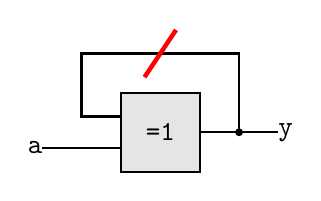
\begin{tikzpicture}[
        font = \ttfamily,
        outer sep = 0mm, inner sep = 0mm,
        comp/.style = {
          rectangle, draw = black, thick, fill = gray!20!white,
          minimum height = 1cm, minimum width = 1cm,
        }
      ]

      \node[comp] (G) {=1};
      \draw[thick] (G.west) ++(0,-.2) to ++(-1,0) node[left] {a};
      \draw[thick] (G.west) ++(0,.2) 
        to ++(-.5,0)
        to ++(0,.8)
        to ++(2,0)
        to ++(0,-1) node[minimum size = 1mm, fill = black, circle] (n) {}
        to ++(-.5,0);

      \draw[thick] (n) to ++(.5,0) node[right] {y};

      \draw[ultra thick, red] (G.north) ++(-.2,.2) to ++(.4,.6);
      % \draw[ultra thick, red] (G.north) ++(.2,.2) to ++(-.4,.6);
    \end{tikzpicture}
  \end{minipage}
\end{center}
but this will be synthesised into an oscillating circuit, that must be avoided
at all costs. The correct way is to have a memory for the next state, with a
logic separated into combinatorial and sequential parts.
\begin{lstlisting}[language=vhdl]
-- combinatorial
y_next <= y xor a;
-- sequential
process (clk)
begin
  if rising_edge(clk) then
    y <= y_next;
  end if;
end process;
\end{lstlisting}
This method is known as \emph{register transfer level} design.

\subsection{Generic Parameters}
Sometimes a group of components have a very similar structure, so instead of
rewriting multiple similar interfaces it is desirable to have \emph{parameters}
and a \emph{generic} entity, for example in the case of a binary counter's
range. To solve the problem using signals with conditional statements would
generate unnecessary hardware, while constants cannot change the entity's port.
Thus there is a syntax:
\begin{lstlisting}[language=vhdl]
generic(
  `\reqph{param name}` : `\reqph{type}` := `\reqph{initial value}`;
  `\optionalph{more parameters}`;
  `\reqph{param name}` : `\reqph{type}` := `\reqph{initial value}`
);
\end{lstlisting}
that has effect at \emph{synthesization time}.

\subsubsection{Generic entity and declaration}
Entities are parametrized as follows.
\begin{lstlisting}[language=vhdl]
entity `\reqph{name}` is
  generic(`\reqph{parameters}`);
  port(`\reqph{pins}`);
end entity `\reqph{name}`;
\end{lstlisting}
For example:
\begin{lstlisting}[language=vhdl]
entity counter is
  generic(CNT_MAX : natural := 127);
  port(
    clk, rst, ena : in std_logic;
    -- adjust to a power of 2
    count : out std_logic_vector(
      (natural(ceil(
        log2(real(CNT_MAX +1)))) -1)
        downto 0);
end entity;
\end{lstlisting}
And in the architecture it is possible to access generic values in a similary
way. Another example is a clock divider.
\begin{lstlisting}[language=vhdl]
entity clockdivider is
  generic(DIV_FACTOR : natural := 128);
  port(...);
end entity;

architecture RTL of clockdivider is
  signal cnt, cnt_next : natural range 0 to (DIV_FACTOR -1);
  ...
\end{lstlisting}

\subsubsection{Generic mapping (Concurrent Area)}
To map a generic entity into a structural design the syntax is extended
accordingly with \vhdl{generic map()}.
\begin{lstlisting}[language=vhdl]
-- definition
component `\reqph{generic entity}` is
  generic(`\reqph{parameters}`);
  port(`\reqph{pins}`);
end component;
\end{lstlisting}
\begin{lstlisting}[language=vhdl]
`\optionalph{label}`: component `\reqph{generic component}`
  generic map(
    `\reqph{parameter}` => `\reqph{constant or parameter}`,
    ...
  );
  port map(
    `\reqph{pin}` => `\reqph{signal or pin}`, 
    ...
  );

\end{lstlisting}

% vim:ts=2 sw=2 et:
